\documentclass[11pt]{article}

\usepackage{svg}
\usepackage{amsmath}

\usepackage{float}

% Setup margins
\usepackage{geometry}
\geometry{
	a4paper,
	top=30mm,
	right=25mm,
	bottom=25mm,
	left=25mm
	}

% Use parskip to leave line between paragraphs as per style
\usepackage{parskip}

% Use fancyhdr package to allow for header style
\usepackage{fancyhdr}

% Standard packages for coloured text, postscript figures (MATLAB figure export)
%  and nice-looking maths
\usepackage{color}
\usepackage{epsfig}
\usepackage{amsmath}
\usepackage{bm}

% Setup caption style
\usepackage[justification=centering]{caption}
\usepackage{subcaption}

% Reduce the itemize item separation
\usepackage{enumitem}
\setitemize{noitemsep}

% Make ``Abstract'' all capitals for style
\renewcommand{\abstractname}{ABSTRACT}

\usepackage{pifont}
\usepackage{cite}
\usepackage{siunitx}
\usepackage[explicit]{titlesec}

\usepackage{multirow}

% Set title and author of document
\title{Fast Prediction of Aerofoil Surface Pressure Distribution using Deep-Learning Techniques}
\author{G. Ai}

\makeatletter
\pagestyle{fancy}
\fancyhf{}
\fancyhead[C]{\small \@author}
\fancyfoot[C]{\thepage}
\makeatother

\renewcommand{\headrulewidth}{0pt}
\renewcommand{\footrulewidth}{0pt}

\titleformat{\section}
  {\bfseries}{\thesection}{1em}{\centering \MakeUppercase{#1}}

\begin{document}
\thispagestyle{plain}

\vspace*{-2cm}

\begin{minipage}[t]{7cm}
\flushleft

\includegraphics{bristolLogo.png}
\end{minipage}
\hfill
\begin{minipage}[t]{7cm}
\flushright
\vspace*{-1cm}
Department of Aerospace Engineering\\
AENGM0032 Research Project\\
2022-2023
\end{minipage}

\vspace{11pt}
\hrule

\makeatletter
\begin{center}
	\vspace{11pt}
	\MakeUppercase{\textbf{\@title}}

	\@author

	Department of Aerospace Engineering, University of Bristol,
	Queen’s Building, University Walk, Bristol, BS8 1TR, UK
\end{center}
\makeatother

\begin{abstract}{\it
For decades, high-fidelity aerodynamic simulations have been an essential part of modern aircraft design. Today, their computational cost is still prohibitively high for iterative optimisation methods. Moreover, as part of a simulation workflow, the meshing process often requires human intervention. This is a significant obstacle that complicates autonomous aerodynamic shape optimisation. In recent years, machine learning techniques have been frequently studied as a promising data-driven surrogate modelling approach to tackle these issues. This research aims to develop a neural network that can predict aerofoil surface pressure distribution in real-time, with similar fidelity to its training data, which are produced by numerical schemes that cost otherwise minutes to compute. The network architecture proposed is a feed-forward, fully connect multi-layer perceptron. The model predictive capability and the implications on their characteristics against model complexity are investigated. Results show that relatively smaller models are sufficiently accurate at subsonic flow regimes, while larger models are required to prevent the smearing of bow shocks at transonic flow conditions.
}\end{abstract}

\begin{center}
	\textbf{Keywords}: deep learning, fast prediction, pressure distribution, aerofoil
\end{center}

\section{Introduction}
\textbf {Aerodynamicists}
 have been working to understand how the shape of aerofoils affects aerodynamic performance since the 20th-century \cite {A.D.Y.1950TheoryIndex.}, by painstakingly conducting wind-tunnel experiments on a range of aerofoils. Despite their high-fidelity results, wind-tunnel experiments are costly and slow to implement. This is a considerable inconvenience for iterative design and optimisation. To speed up the design process, numerical methods complemented with empirical models were used instead \cite {Drela1987Viscous-inviscidAirfoils}.
 
Penal methods and coupled Euler methods are low-fidelity schemes that enable fast prediction. Xfoil \cite {Drela1989XFOIL:Airfoils.}, for example, still remains to be a useful tool for rapid prediction of low incidence aerofoil performance at a certain range of Reynolds number and low speed (i.e., negligible compressibility effect). To gain higher fidelity results while still avoiding the cost of wind-tunnel experiments, Reynolds-averaged Navier-Stokes (RANS) simulation is routinely utilised in modern aerodynamics research and aircraft design. Nonetheless, mesh generation requires prior knowledge of likely results and the computing time for a single high-resolution simulation tends to be long.

Nowadays, with new technologies such as virtual reality and meta-verse emerging, most pilot training may rely on realistic flight simulators that are cheaper, safer, and more accessible. The aviation community is in desperate need of a fast and accurate model, for predicting the forces and moments acting on aerofoils, which can hopefully be generalised to 3D wings and even the whole aircraft. If such a model existed, there could be a next generation of highly realistic flight simulators that enjoy this real-time high-fidelity aerodynamics in nonlinear flow regimes often occurring at stall or when fighters perform aerobatics such as the ‘cobra manoeuvre’.

The aim of this study is to investigate the speed and accuracy of using deep neural networks (DNNs) as a surrogate model of high-fidelity physics-based simulations.

\section{Background}
The industry used to highly rely on wind tunnel testing and flight tests, which were merely complemented by Computational Fluid Dynamics (CFD) to decrease testing hours and the number of test entries \cite {Jameson1999Re-engineeringComputation}. But nowadays, wind tunnel data is only required to complement and validate CFD results \cite {Malik2012RoleRD}. There are even situations where CFD is used exclusively, when the product model is too complex or when the flow conditions exceed wind tunnel capabilities, e.g., re-entry in hypersonic flows of fluid with exotic chemical composition \cite {Wright2010AMissions}. Current use of simulations in aerospace industries varies with the type of vehicle, flight conditions, and components in question. Low-fidelity CFD codes are widely adopted in conceptual design to trade off the modelling accuracy of flow physics for higher throughput. However, more frequent use of high-fidelity CFD codes in detailed design is restricted by the associated mesh generation effort and long computing time.

In general, accuracy and speed are the two factors that limit the widespread adoption of simulations across design phases \cite {Slotnick2014CFDAerosciences}. Industrial CFD codes face several challenges: e.g., high dimensional strain tensor due to 3D boundary layers; shock and junction induced boundary layer separation; vortical structures from vortex generators interacting with boundary layers. One of the key limitations of physics-based simulations that challenged their accuracy is turbulence modelling. The turbulence models \cite {Wilcox1993TurbulenceCFD} used in steady RANS are effective with attached flows but fail to capture the physics at the outer flow field as compared to LES. As a great combination, DES is both computationally cheaper and more accurate with respect to either of the pure formulations. But this technique can be less accurate than RANS when the wall-parallel grid spacing is close to the boundary-layer thickness \cite {Spalart2008Detached-EddySimulation}. Because most CFD codes involve much empiricism in their boundary layer formation, there has been no generalised definition for turbulence transition in current CFD methods.

With wider utilisation of graphic processing units for tensor manipulations and more accessible high-performance parallel computing facilities, the actual running time of a high-fidelity CFD code will eventually become less of a problem. However, it is the geometry pre-processing and mesh generation stages that are increasingly felt as bottlenecks in accelerating modern CFD workflows. Automated mesh generation for even regular components will result in high software complexity and still suffer from inadequate robustness when dealing with novel configurations, i.e., the location of flow features such as shocks, wakes, and shear layers are not known in advance. This issue resulted in the difficulty to eliminate human intervention in simulation processes \cite {Cary2021CFDPerspectives}.

During the past decade, the development of advanced surrogate modelling techniques \cite{Forrester2007Multi-fidelityModelling, Bouhlel2019ADerivatives} has enabled fast and automated implementation of simulation data in aerodynamic optimization of aerofoil and aircraft \cite{Bevan2017AdaptiveGeometry}. Forrester et al. demonstrated a multi-fidelity wing optimization using Gaussian process \cite{Forrester2008EngineeringModelling}. Proper orthogonal decomposition was utilised in an evolutionary optimization of aerodynamic design \cite{Iuliano2013ProperDesign}. Variable parameterization and corrected space mapping were introduced by Robinson et al. \cite{Robinson2008Surrogate-BasedMapping} who achieved 76\% savings in high-fidelity function calls. Mackman et al. \cite{Mackman2013ComparisonModels} compared various adaptive sampling methods to construct surrogate aerodynamic models. Surrogate modelling is a subset of metamodeling techniques, which were reviewed by Viana et al. \cite{Viana2014SpecialCome} to examine their use in multidisciplinary optimization. As an example of ongoing development, machine learning (ML) methods have seen an increase in aerodynamic research over the years \cite{Sun2019ADesign}. This development has enabled more generalised surrogate modelling techniques in fast optimisation based on high-fidelity data.

ML algorithms, particularly Deep Neural Networks (DNNs), have gained much success in computer vision and natural language processing in recent years. Suddenly, there has been a massive spike in many industries to implement this kind of algorithm that automate tasks traditionally done manually. Surprisingly, ML is not at all a new idea. Rosenblatt \cite{Rosenblatt1958TheBrain} proposed the first learning machine called perceptron that performs classification and regression. Although Minsky et al. \cite{Minsky1988PerceptronsGeometry} showed that a single layer of neurons, i.e., the perceptron, is not capable of learning nonlinear functions and most certainly cannot approximate any function, e.g., the XOR function, it is now known that a multilayer DNN is essentially a universal function approximator \cite{Brunton2020MachineMechanics}, provided that enough dense layers with adequate number of neurons are stimulated by appropriate (nonlinear) activation functions.

ML, or its premature form i.e., statistical learning theory, has actually met with aerodynamics even before NACA produced the first systematic theory of wing sections. It was first introduced by Kolmogorov \cite{Kolmogorov2010TheNumbers} who claimed that one of its practical applications is turbulence modelling. Unfortunately, it was not until a few decades later that ML properly crossed paths with fluid mechanics. Baldi et al. \cite{Baldi1989NeuralMinima} were the first to draw the link between single-layer autoencoders (unsupervised linear NNs) and proper orthogonal decomposition (POD) to extract the first few primary modes of turbulence flow fields. Later, DL also had its debut in the field of fluid mechanics in the form of a deep autoencoder for reconstructing the boundary region of a channel flow \cite{Milano2002NeuralFlow}.

Perhaps, one of the most well-known DL algorithms today is Convolutional Neural Networks (CNNs) \cite{LeCun1989HandwrittenLearning}, which have been playing a vital role in modern society and are powerful algorithms for object detection and image segmentation, or when dealing with any kind of high-dimensional inputs with a grid-like topology \cite{Bhatnagar2019PredictionNetworks}. Although a feed-forward fully connected NN is, in principle, also capable of feature extraction, the associated number of neurons, thus, trainable parameters become impractically large during backpropagation \cite{Rumelhart1986LearningErrors}. One special type of CNN called U-net \cite{Ronneberger2015U-Net:Segmentation} is a fully convolutional network that also outputs images. Their architecture resembles a kernel version of autoencoders and is particularly useful for mapping an input image to a target image. This character comes in handy for predicting RANS solution over an aerofoil as the pressure and velocity components maps are essentially image-like data with high dimensionality and grid-like topology. Theurey et al. \cite{Thuerey2020DeepFlows} utilised a U-net that directly takes the boundary conditions for a RANS solver as input and succeeded in their attempt to map the boundary conditions to an inferred steady-state flow field within 3\% of mean relative error. Similarly, Yang et al. \cite{Yang2022FlowfieldAutoencoder} modified an autoencoder to predict off-design flow fields of aerofoils based on those computed by RANS at cruise point. They claimed a 30\% reduction in prediction error compared to generic autoencoders and implemented physics-guided training to improve the model’s generalisability. Physics-informed ML (PIML or PINN) was proven by Ling et al. \cite{Ling2016ReynoldsInvariance} to be an efficient strategy to incorporate invariances and symmetries derived from first principles. It not only improves model accuracy and, in some situations, training rate, compared to traditional ML techniques when data is sparse, but also fosters the models’ ability when extrapolating \cite{Wang2017Physics-informedData, Raissi2019Physics-informedEquations}.

The objective of this study is to develop a feed-forward dense neural network that predicts surface pressure distributions over common aerofoils and compare it with a similar approach \cite{Sabater2022FastTechniques} done very recently. The key difference is that their model predicts the pressure coefficient on one point of the surface at a time, whereas this study intends to output a whole surface pressure distribution in one inference. The preparation of datasets, multi-output regression DNN architecture and optimizer are presented in Sec. III. The predictive capability of the purposed model is presented in Sec. IV.\\
\\

\begin{figure}[htbp]
    \centering
    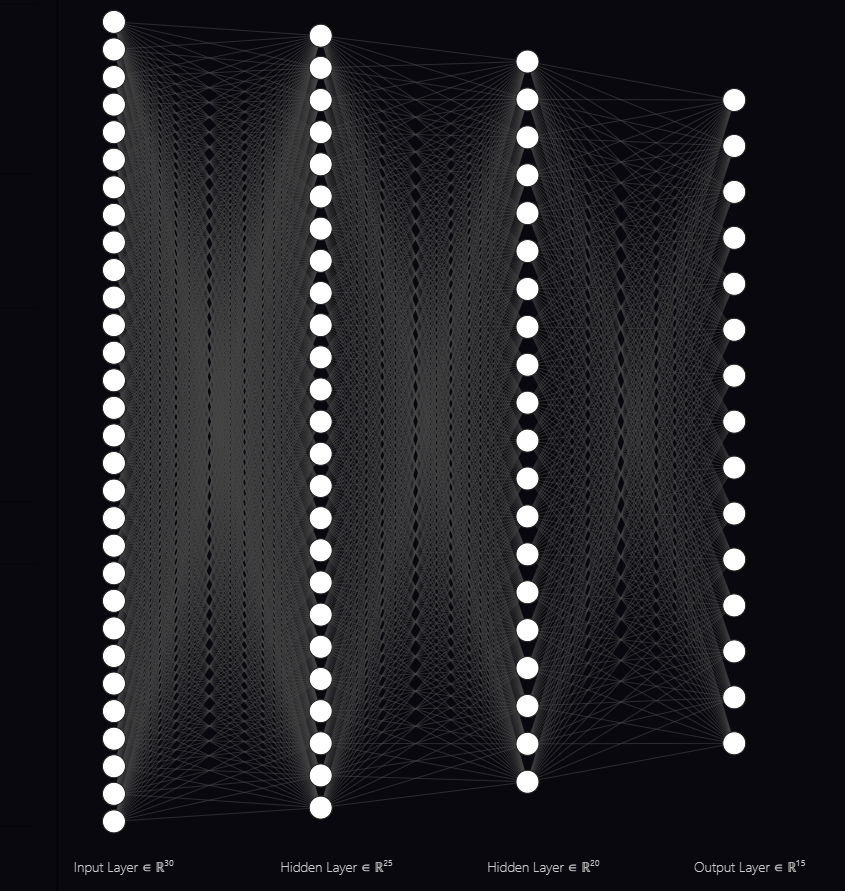
\includegraphics[scale=0.71]{Architecture.png}
    \caption{Typical architecture of a feed-forward fully connected dense neural network. Note that the layer size is not to scale as most pressure distribution comprise more than a hundred pressure tappings.}
\end{figure}

\section{DNN for Pressure Prediction}

The proposed surrogate model is essentially a data-driven method for predicting the distributed quantity of interest. It is assumed that a proper CFD analysis can be described as a full-order model (FOM) function:

\begin{equation}
	\label{eqn:1}
	\begin{split}
        \hm{Cp} &= f( \hm{x}, \hm{y}, \hm{\theta} ) \\
	\end{split}
\end{equation}

where $\hm{Cp}$ is an array of distributed aerofoil surface pressure coefficients, $\hm{x}$  and $\hm{y}$ describes the geometry of an aerofoil, and $\hm{\theta}$ denotes the flow conditions, i.e., Reynolds number, angle of attack and Mach number. The DNN serves as an approximated substitution of the FOM. A trained DNN is expected to predict data with similar fidelity as the FOM, but entails much less computational cost and, most importantly, eliminates the need for human intervention to generate a mesh.

\subsection{Formulation}

For a general aerodynamic problem, the simulation is expected to output the surface pressure coefficient at the location of each input surface geometry point. This means the length of the model input array is at least twice that of the model output array for 2D problems, and triple for 3D problems. To reduce the number of DNN parameters so the model complexity is manageable, the input geometry is represented by intermittent points on the aerofoil surface such that the number of DNN input nodes is the same as the number of output nodes.

In the case of inviscid simulations, the flow condition vector can be reduced to a 2D vector such that

\begin{equation}
	\label{eqn:2}
    \hm{\theta} =
    \left[ {\begin{array}{cc}
    incidence \\
    Mach ~ number \\
    \end{array} } \right]
\end{equation}

where Mach number can be interpreted as 0 for incompressible cases, thus justifying an option to further reduce the $\hm{\theta}$ vector to a scalar when training with data from the vortex panel method as the FOM. However, note that Reynolds number is infinite for inviscid flow. Consequently, unlike the Mach number which can either be zero or omitted as input, the Reynolds number must be excluded from the $\hm{\theta}$ vector when the DNN is learning solutions of potential flow or Euler equations.

\subsection{Deep-Learning Technique}

The dataset is prepared as follows:

\begin{itemize}
    \item Training data: NACA aerofoils at a range of flow conditions. They are a common set of aerofoils that enjoy a very systematic parameterisation method which allows ease in the preparation of a large number of training entries.
    \item Validation data: NACA aerofoils with changed parameters and flow conditions in between those in the training data. The DNN is set to minimise the loss in the validation data during training, thus validating its ability to interpolate between taught flow conditions. The geometries are not exactly the same as those in the training data, but they share the same parametrisation method.
    \item Testing data: RAE2822 aerofoil at unseen flow conditions. This should also provide insight into the generalisability of the deployed DNN with untaught geometries. Since variation in flow conditions can be easily pre-considered for the DNN, whereas geometries cannot, this is why training and validation geometries were intentionally kept similar, while the DNN is tested with a new aerofoil that shares no commonality in the parametrisation method of NACA aerofoils.
\end{itemize}

\begin{figure}[htbp]
    \centering
    \includesvg[scale=0.5]{c0t9}
    \caption{Geometries of NACA aerofoils (blue) and RAE2822 aerofoil (red).}
\end{figure}

The DNN architecture under investigation is one of the earliest models that emerged with the field of ML. It is the most basic, yet powerful algorithm that is able to extract and utilise the underlying coherent structures in a given set of training data. The DNN relies on the information obtained from the actual solutions of the FOM to infer the behaviour of the FOM at new conditions. Starting with the first layer of neurons, the output of each neuron is a weighted sum of the input data with an added bias and is passed through an activation function before it is fed to each neuron in the next layer.

\begin{equation}
	\label{eqn:Example}
	% Use split for multiline equations.
	% It only supports one alignment point (&), generally placed by the equals
	\begin{split}
        output_n = ReLU(~ bias_n + \sum_{i=1}^{length(input)} & input_i \times weight_i ~) \\
		n \in [1, number~of~nodes], ~& and ~ n \in N
	\end{split}
\end{equation}

Where the output array of the previous layer is the input array of the next layer. Each neuron stores an array of the weights for the corresponding outputs of the previous layer. It also stores a scalar bias which applies an offset to the dot product between its inputs and its weight array. The activation function is chosen to be rectified linear activation function (ReLU), a piecewise linear function that will output the input directly if it is positive, otherwise, it will output zero. Note that a bias can effectively be interpreted as a horizontal shift to the plot of an activation function.

\subsection{Implementation $\And$ Optimisation}

The training algorithm, i.e., backpropagation, aims to minimise the root mean square error (RMSE) between the model output and supplied ground truth by adjusting the weights and bias in the neurons, using stochastic gradient descent with information from the first derivative of the chosen activation function. Adam optimiser \cite{Kingma2015} is the chosen algorithm for its outstanding convergence performance and versatility, while requiring little tuning on training parameters. It autonomously adjusts the learning rate during training. And the only parameter that needs to be specified beforehand is the initial learning rate, which is a constraint to the highest learning rate allowed among all the neurons. This approach is implemented in Python, using the TensorFlow \cite{tensorflow} library with the Keras \cite{Chollet2015} backend.

The hyperparameters tuneable are the number of layers in the DNN model and the initial training rate of the Adam optimiser. The objective is to obtain the most efficient number of hidden layers in the DNN where model performance against model size stagnates. The model performance is measured by the least accurate inference on the testing data, i.e., the prediction that results in the highest RMSE. The initial learning rate is heuristically tuned such that the initial loss is not too high to cause a drastic decrease of learning rate \cite{Reddi2018} computed in the Adam algorithm, while still being reasonably efficient in terms of convergence over epochs.

\section{Predictive Capability}

This section investigates the model performance and training costs against model complexity. The systematic behaviour of the models and their implications are analysed and discussed. To gain insights into the performance and characteristics of the models in a production setting, the discussed results below are produced from testing data, which have not been seen by any model before.

\subsection{Inviscid Incompressible Flow}

The result from tunning the hyperparameters of the DNN model has been tabulated in Table 1, where each layer is comprised of 256 nodes.

\begin{table}[H]
	\centering
	\caption{Effect of layer number to the model performance and training cost.}
	\label{tab:Example}
	\begin{tabular}{cccc}
		\hline
		Number of Layers & Mean RMSE & Training Time & Learning Rate \\ \hline
		DNN-8     & 0.009914 & 4ms/step & 10e-3       \\
		DNN-7     & 0.009991 & 3ms/step & 10e-3       \\
		DNN-6     & 0.010498 & 3ms/step & 10e-3       \\
		DNN-5     & 0.011276 & 3ms/step & 10e-4       \\
		DNN-4     & 0.012070 & 2ms/step & 10e-4       \\
		DNN-3     & 0.021139 & 2ms/step & 10e-4       \\ \hline
	\end{tabular}
\end{table}

It is obvious that training cost grows as number of layers increases. It was not foreseen though that as number of layers attenuates, it is better to decrease the initial learning rate to achieve a smooth decrease in the loss history. In fact, it has been observed that excessive learning rate can cause the optimizer to be stuck at a higher local minimum than it could have achieved with a more conservative initial learning rate.

Loss function is calculated as the average RMSE between predictions and ground truths of all training entries. Best initial learning rate is decided when the loss history shows a typical exponential decay over epochs. Figure 3 shows that the loss has converged in the last 20 epochs.

\begin{figure}[htbp]
    \centering
    \includesvg[scale=0.75]{history}
    \caption{Loss history of the best model DNN-8.}
\end{figure}

DNN-3 yields a much higher mean RMSE than most of the other models, while the mean RMSE of DNN-4 enjoys a significant drop compared to more complex models without sacrificing too much training cost. The DNN-4 model is already capable of predicting results of linear continuous FOM with acceptable accuracy. Results from the worst prediction are plotted in Figure 4 and 5.

\begin{figure}[H]
    \centering
    \includesvg[scale=0.75]{scatter}
    \caption{Scatter plot of predicted Cp against ground truth.}
\end{figure}

It can be seen from Figure 4 that a few pressure prediction points are consistently underestimated. They turn out to be at the suction peak of the Cp plot (Figure 5). As the suction peak is where the pressure varies most against angle of attack, it is expected that this region will be least accurate. The flow condition in this subsection is angle of attack alone. The training (seen) incidences, and validation or testing (unseen) incidences are chosen as below.

\begin{equation}
	\label{eqn:Example}
	% Use split for multiline equations.
	% It only supports one alignment point (&), generally placed by the equals
	\begin{split}
        seen~incidences~=~n-10,~~~~where~n\in[1,20]~and~n\in N \\
		unseen~incidences~=~n-2.5,~~~~where~n\in[1,5]~and~n\in N
	\end{split}
\end{equation}

where $N$ is the set of natural numbers.

\begin{figure}[htbp]
    \centering
    \includesvg[scale=1.0]{WorstPrediction}
    \caption{Comparison between prediction and true pressure distribution.}
\end{figure}

The models gain more predictive capabilities about suction peak when layer size is increased. Results show that DNN-8 model can predict suction peaks much more reliably. The worst prediction and an average prediction from DNN-8 are shown as below. Both the worst the average inferences provide faithful prediction of the location and strength of the suction peaks.    \\
\\
\\

\begin{figure}[htbp]
    \centering
    \includesvg[scale=0.9]{BWP}
    \caption{The worst prediction by DNN-8.}
\end{figure}

\begin{figure}[htbp]
    \centering
    \includesvg[scale=0.9]{BAP}
    \caption{An average prediction by DNN-8.}
\end{figure}

\subsection{Inviscid Compressible Flow}

Below is the result from tunning the hyperparameters of the DNN model. Note that training took place on a different platform thus, training rates in Table 1 and 2 are incomparable between each other. Number of epochs is increased to 500 to ensure convergence.

\begin{table}[H]
	\centering
	\caption{Effect of layer number to the model performance and training cost.}
	\label{tab:Example}
	\begin{tabular}{cccc}
		\hline
		Number of Layers & Mean RMSE & Training Time & Learning Rate \\ \hline
		DNN-11    & 0.099372 & 8ms/step & 10e-3       \\
		DNN-10    & 0.100276 & 7ms/step & 10e-3       \\
		DNN-9     & 0.134562 & 7ms/step & 10e-3       \\
		DNN-8     & 0.178634 & 6ms/step & 10e-3       \\
		DNN-7     & 0.237809 & 6ms/step & 10e-4       \\
		DNN-6     & 0.273897 & 5ms/step & 10e-4       \\ \hline
	\end{tabular}
\end{table}

DNN-11 was chosen as the model to further investigate. Here, it is hard to choose the best one in terms of model efficiency. The author found that the more layers added, the more accurate the model tends to be. It is decided that the hyperparameter study conclude at this point as adding more layers makes training time unmanageable and real-time inference problematic.

The flow conditions are chosen as
\begin{equation}
	\label{eqn:Example}
	% Use split for multiline equations.
	% It only supports one alignment point (&), generally placed by the equals
	\begin{split}
        seen~Mach~number=0.6+0.02m,~~~~&unseen~Mach~number=0.61+0.02m\\
        where~m\in[0,19]~&and~m\in N \\
		seen~incidences=-0.5+0.2n,~~~~&unseen~incidences=-0.4+0.2n\\
        where~n\in[0,4]~&and~n\in N
	\end{split}
\end{equation}
where $N$ is the set of natural numbers.

Figure 8 indicates that the transonic regime is harder to predict than flow conditions where weak or no bow shock occurs on the aerofoil surface. The local minimums in this plot are caused by angle of attacks that results in weaker bow shocks. The worst prediction is the one where shock strength is at the highest. Moreover, as Mach number is increased further so that oblique shock forms on the aerofoil surface, the RMSE drop back to a similar level as where Mach number is not high enough to form bow shocks.

\begin{figure}[htbp]
    \centering
    \includesvg[scale=0.62]{RMSE}
    \caption{RMSE between prediction and ground truth against Mach number.}
\end{figure}

\begin{figure}[htbp]
    \centering
    \includesvg[scale=0.75]{smeared}
    \caption{Pressure distribution on the lower surface of NACA1812.}
\end{figure}

\begin{figure}[htbp]
    \centering
    \includesvg[scale=0.75]{bestShock}
    \caption{Best shock prediction by DNN-11.}
\end{figure}

In Figure 9, most pressure prediction is very accurate, apart from a smeared shock predicted by the DNN-11 model. In fact, this is a very typical phenomenon displayed in most predictions where bow shocks are involved.

One of the best shock predictions by DNN-11 is plotted in Figure 10. Other DNN models with a smaller number of hidden layers were not able to predict shock as good as DNN-11.

To further investigate the impact of smeared shock in pressure curve to the overall lift coefficient, the lift coefficient on the lower surface of the aerofoil (referred to as suction from now on) is calculated and tabulated below. The error of suction between predicted (smeared) and true pressure distribution is considered low.

\begin{table}[H]
	\centering
	\caption{Comparison between the error derived from the integrated quantities computed from prediction and ground truth.}
	\label{tab:Example}
	\begin{tabular}{cccc}
		\hline
            & Suction & Prediction & Error \\ \hline
		Case No.62    & 9.193     & 8.793     & 0.310    \\
		Case No.68    & 13.544    & 13.292    & 0.252     \\ \hline
	\end{tabular}
\end{table}

In terms of geometry generalisability, the results are much less optimal. Previous predictions are done on familiar geometries. When testing with RAE2822 instead of a NACA aerofoil, the predicted pressure distribution looks significantly like those of NACA aerofoils, showing an indication of overfitting of the model to training data. It can be seen from Figure 11 and 12 that both the worst and best predictions are below acceptable accuracy.

\begin{figure}[htbp]
    \centering
    \includesvg[scale=0.75]{rae}
    \caption{The worst prediction on RAE2822.}
\end{figure}

\begin{figure}[htbp]
    \centering
    \includesvg[scale=0.75]{bestRAE}
    \caption{Best prediction on RAE2822 with NACA aerofoils as training data.}
\end{figure}

\section{Conclusions}

Deep learning techniques, particularly multilayer perceptron, have been utilised to reduce the cost and inconvenience when iteratively predicting aerodynamic quantities, in this case, pressure distribution is the subject. Note that surface friction distribution can also be predicted by a similar manner. In contrary to other DNN architectures, e.g., CNN and autoencoders, the predictive accuracy and characteristics of fully connect feedforward dense neural network models have been investigated with varying number of layers.

For inviscid incompressible cases, the predictions produced by DNN-4 are satisfactory, with highest efficiency in terms of accuracy over model complexity. Additionally, DNN-8 can predict suction peaks much more precise than other models that have a smaller number of layers. For compressible cases, strong local effects, e.g., bow shocks that occur at the transonic regimes, can still be smeared even when using the largest model DNN-11.

Moreover, when the best trained model encounters a completely new geometry with exotic parametrisation methods that are different from those of the training data, its prediction becomes highly unreliable as the model does not possess knowledges from enough similar geometries to interpolate between.

In fact, it is possible to improve the model capability by increase the number of layers. Results shown that a very large model (DNN-11) was able to produce less smeared pressure curve and, in some cases, faithfully predict both shock strength and position. When the model has predicted shock position correctly, the error of integrated force coefficient between prediction and ground truth are extremely similar, meaning that the model is still highly useful and accurate so long as only the integrated quantities are of interest.

Most models can be evaluated in real-time, thus allowing their applications in time-critical tasks that require high-fidelity aerodynamic data. In general, apart from the long training time associated with deep learning techniques, the proposed approach has its potential in real-time high-fidelity aerodynamic data predictions under unseen flow conditions, given that it is implemented on similar geometries which share one parametrisation method.

\section{Further work}

To improve the difficult prediction of bow shocks encountered at transonic regimes, another network dedicated to predicting the two quantities, i.e., shock strength and shock location, was developed and tested, but yields unsatisfactory results. Further investigations on the influence of other back propagation algorithms and various activation functions to the ability of the optimizer to converge to a lower local minimum can be the next step to help better understand and identify the best model configuration for this task.

% For a separate BibTeX file, use the commands below instead of
%  the `thebibliography' section
% Set to IEEE style
\bibliographystyle{ieeetr}
% Get the references from references.bib
\bibliography{reference}


\end{document}